\documentclass[12pt,righttag]{article}

\usepackage{amssymb}
\usepackage{graphicx}

\begin{document}
	\title{A Numerical Investigation of Poisson's Equation}
	\author{Sean Sweany}
	\renewcommand{\today}{February 12, 2016}
	\maketitle
	
	\section{Introduction}
	Poisson's equation is a partial differential equation used in describing everything from the electric potential of a charge distribution to gravitational fields. Our goal here is to go and take an equation that has a known analytical solution to Poisson's equation and write a code to numerically solve said equation. Once a working code is complete the next step is to investigate the error that comes from the numerical method being used as well as how our code compares to other methods of solving it in terms of performance.
	
	\section{Numerical Methods}
	Poisson's Equation can be written as:
	\[\bigtriangledown^2\rho=-f(x)\]
	For this project Poisson's equation will only be solved in one dimension so the del square reduces down to just the second derivative of $\rho$. Now, taking the function $\rho$ and expanding it as a Taylor series, with some algebraic manipulation (we did this in class and it really doesn't provide much insight, it is simply some nice little algebraic manipulation) the following equation can be obtained for the second derivative of said function:
	\[\bigtriangledown^2\rho=-\frac{\rho_{i+1}+\rho_{i-1}-2\rho_i}{h^2}\]
	Now, looking at this equation it is easy to see that it can be made into a matrix with 2 on the diagonal and -1 on the off diagonals multiplied by a vector. Using this it is now possible to turn this nice little equation into the following:
	\[Ax=b\]
	By finagling Poisson's equation into this cute little form it makes it very easy to solve using Gaussian Elimination. However, in the words of the late Billy Mays "But wait there's more," and yes their is more. Mainly, that since the matrix being worked with is sparse with 1's on the off diagonals we can actually solve the problem using 3 vectors. One for the whole A matrix, one for x and one for b. Now, claiming that A can be made into a matrix may not seem like the most natural thing to do at first but it is actually a much easier and faster way to go about solving the problem.
	
	So the algorithm to solve Poisson's equation will then have, for the forward elimination:
	\[a_{[i+1]}=a_{[i+1]}-\frac{1}{a_{[i]}}\]
	\[b_{[i+1]}=b_{[i+1]}-b_{[i]}\frac{1}{a_{[i]}}\]
	where the a's are for the diagonal matrix elements and the b's come form the adjustments to what is trying to be solved for caused by the Gaussian elimination, after solved the a's and b's are then stored in vectors. Next is the backward substitution, this will not affect the matrix elements however it will affect the vector b.
	\[b_{[j-2-i]}=b_{[j-2-i]}-b_{[j-1-i]}\frac{1}{a_{[j-1-i]}}\]
	In this equation j is the size of the matrix we are working with. Solving Poisson's equation like this is very efficient, using only 8n FLOPS. Now, comparing this to the regular Gaussian elimination method which takes on the order of $\frac{2}{3}n^3$ flops, and LU decomposition even takes the order of $n^3$ flops to decompose the matrix into the upper and lower parts. However, once decomposed solving only takes $n^2$ flops.
	
	 The nice thing about this three vector method of solving the equation is that later if there are any other tridiagonal matrices where the off diagonal elements are not 1 then it is easy to add in two more vectors and change the 1's to the corresponding vector components multiplied together. Now, it does come with the disadvantage that it is not as fast as some other algorithms. However, later on it will become apparent that this method is more than fast enough and using a faster method would only save a second or so, which in my opinion is less useful than having a code that can easily be modified for other situations.
	
	Poisson's equation is nice since it only has 1's and 2's along the diagonal, the thing is though these methods for solving linear equations can run into problems. One problem arises if there are zeros in the line which you are trying to eliminate elements from. To deal with this sort of issue some sort of pivoting algorithm would have to be applied to the matrix rows. To pivot all one has to do is take the problematic row and move it down in the matrix to a place where the zero will actually help with the Gaussian Elimination or LU decomposition which is being preformed. Another issue that can come about in this code is choosing an incorrect step size. To large a step size and the error will be introduced into the solution, but if it is too small then round off error will accumulate as well as your code will take much longer to run.
	
	\section{Results and Discussion}
	
	For this project the equation being solved for with Poisson's Equation was:
	\[f(x)=100e^{-10x}\]
	Which has the analytical solution:
	\[u(x)=1-(1-e^{-10})x-e^{-10x}\]
	Dirichlet Boundary conditions were enforced and the equation was solved in the space from 0 to 1. Data was taken for matrices of sizes 10 by 10, 100 by 100 and 1000 by 1000, each of these matrices correspond to step sizes of $\frac{1}{n+1}$. Along with these, the code was also able to run matrices whose size was on the order of $10^7$. What the different matrix sizes represent is different step sizes since for all of this project we are only solving Poisson's equation in the range from 0 to 1. Below in figure 1 are the solutions for the three sizes matrices mentioned above. It is apparent that for the 10 by 10 matrix the solution differs quite a bit from the actual solution. For a 100 by 100 matrix though just by eye it appears as though the solution has converged to the true solution.
	
	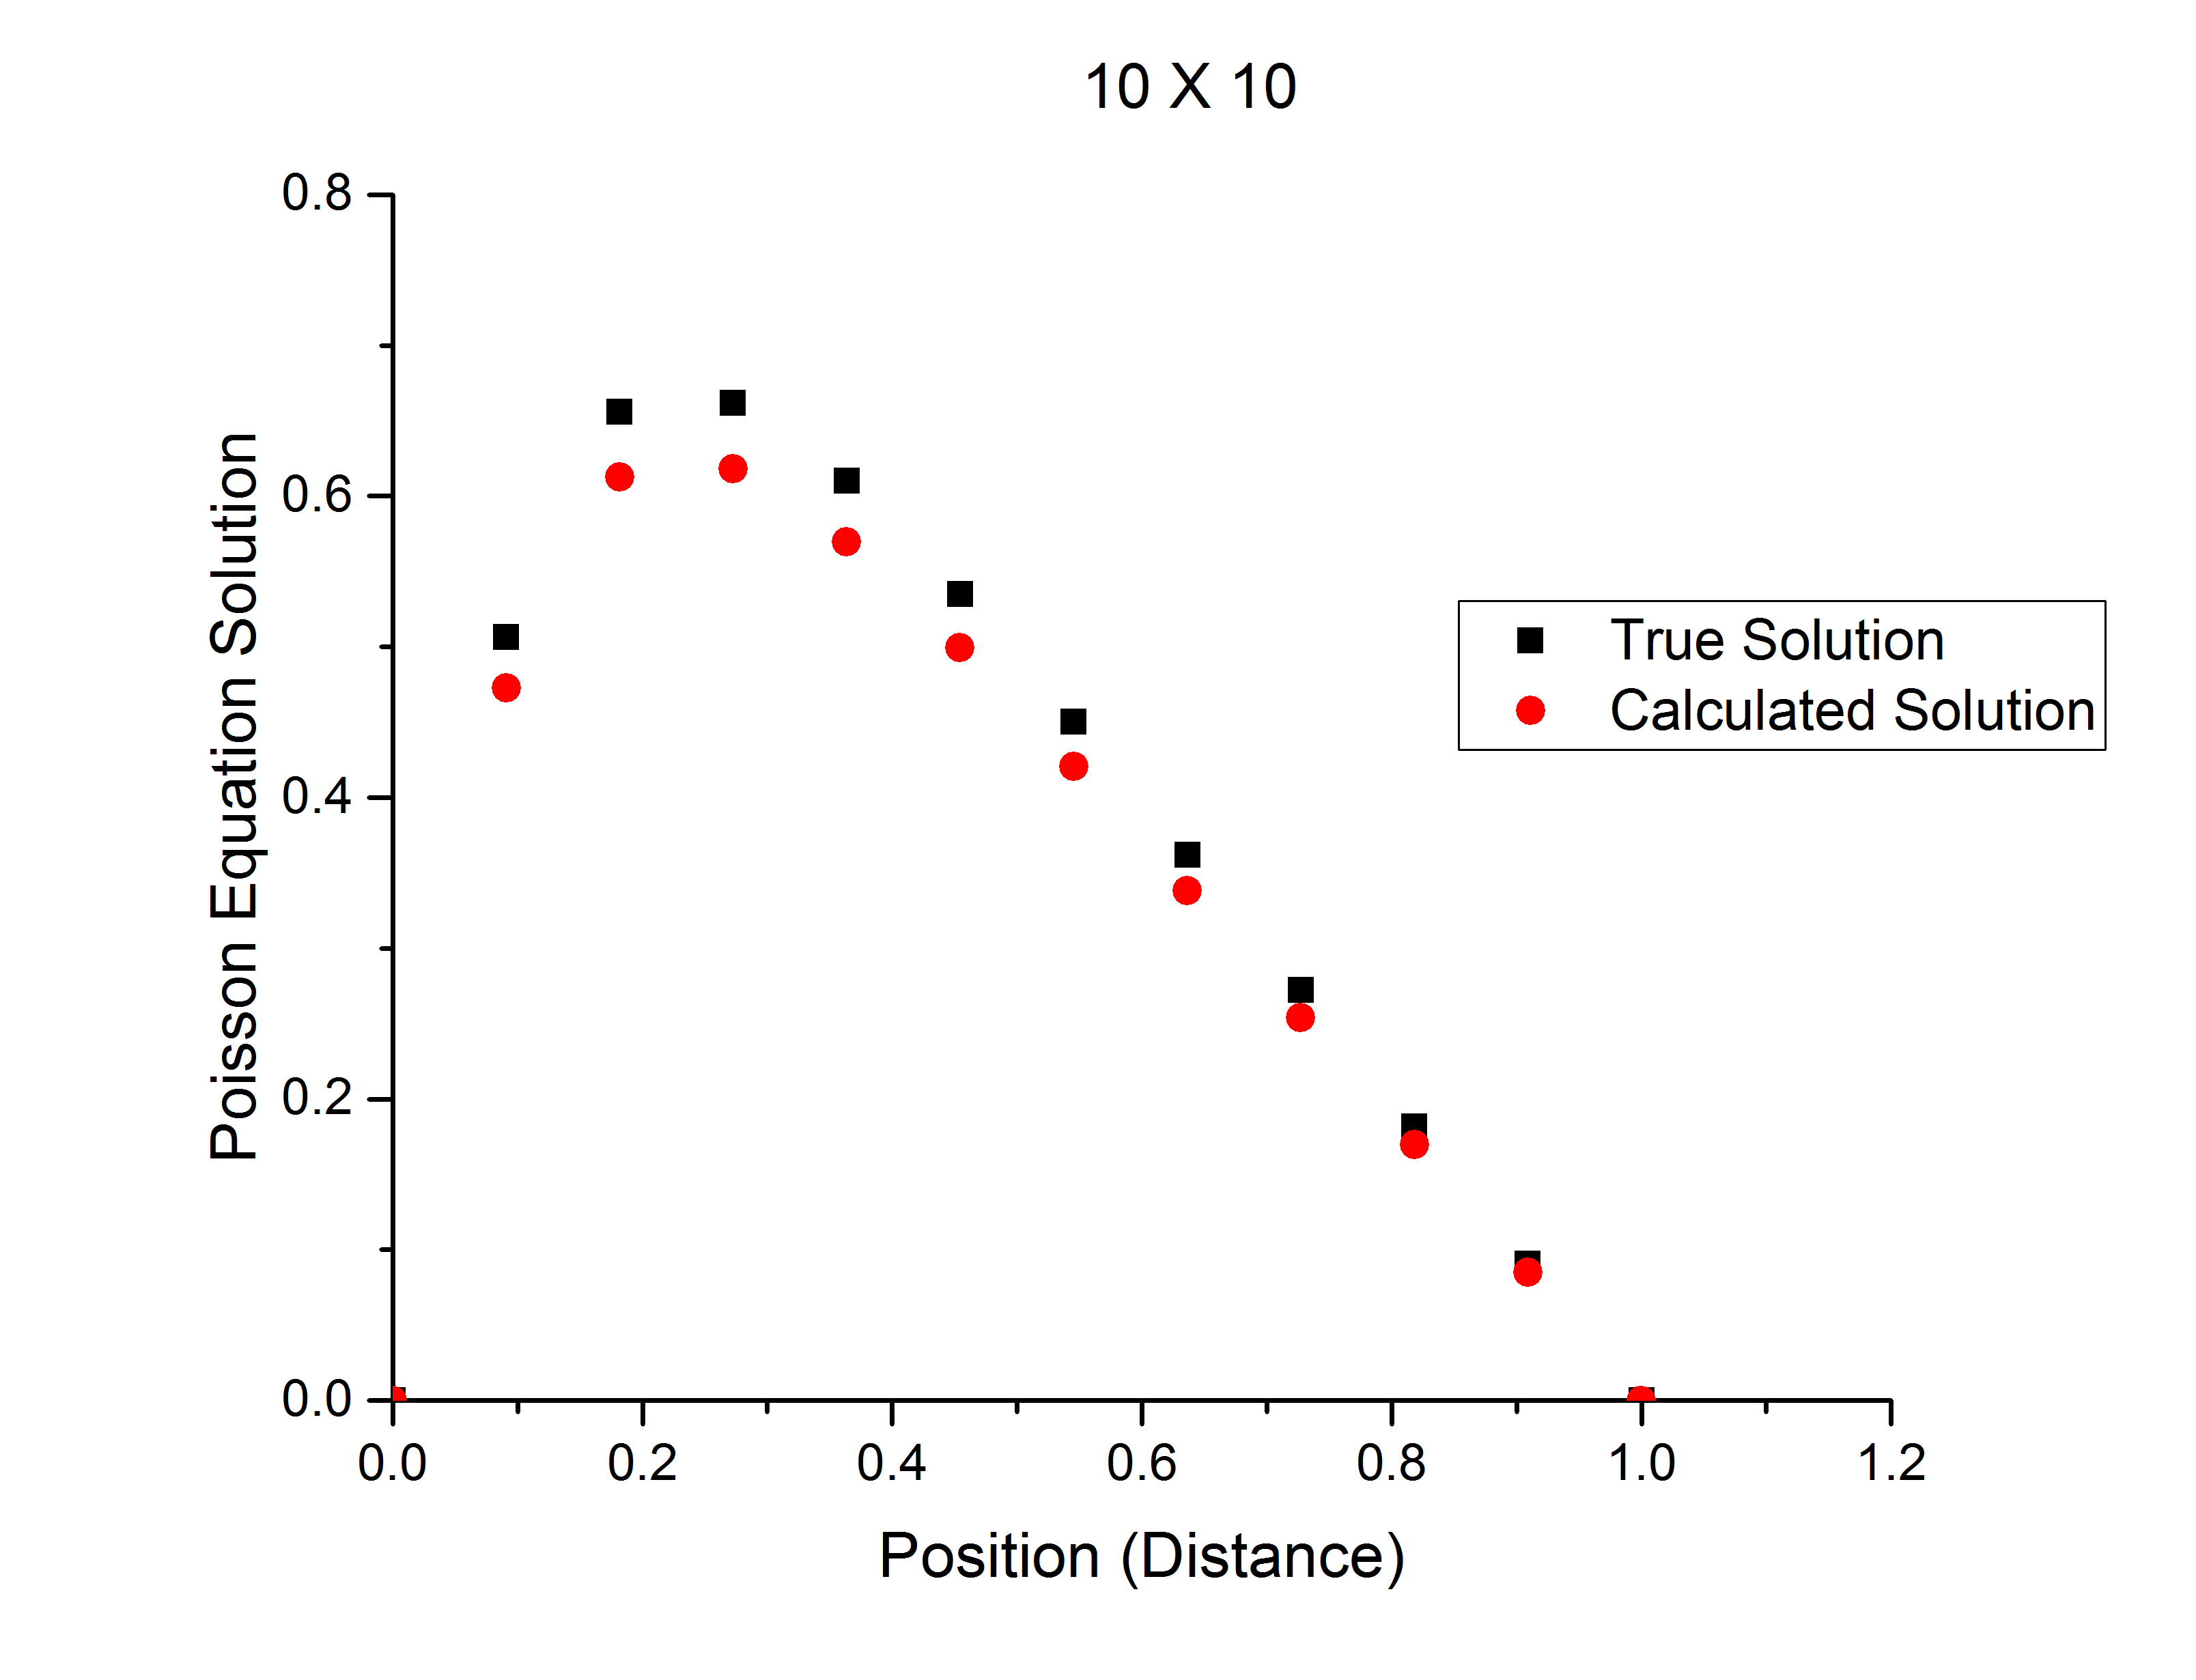
\includegraphics[scale=0.25]{10GridPoisson.png} 
	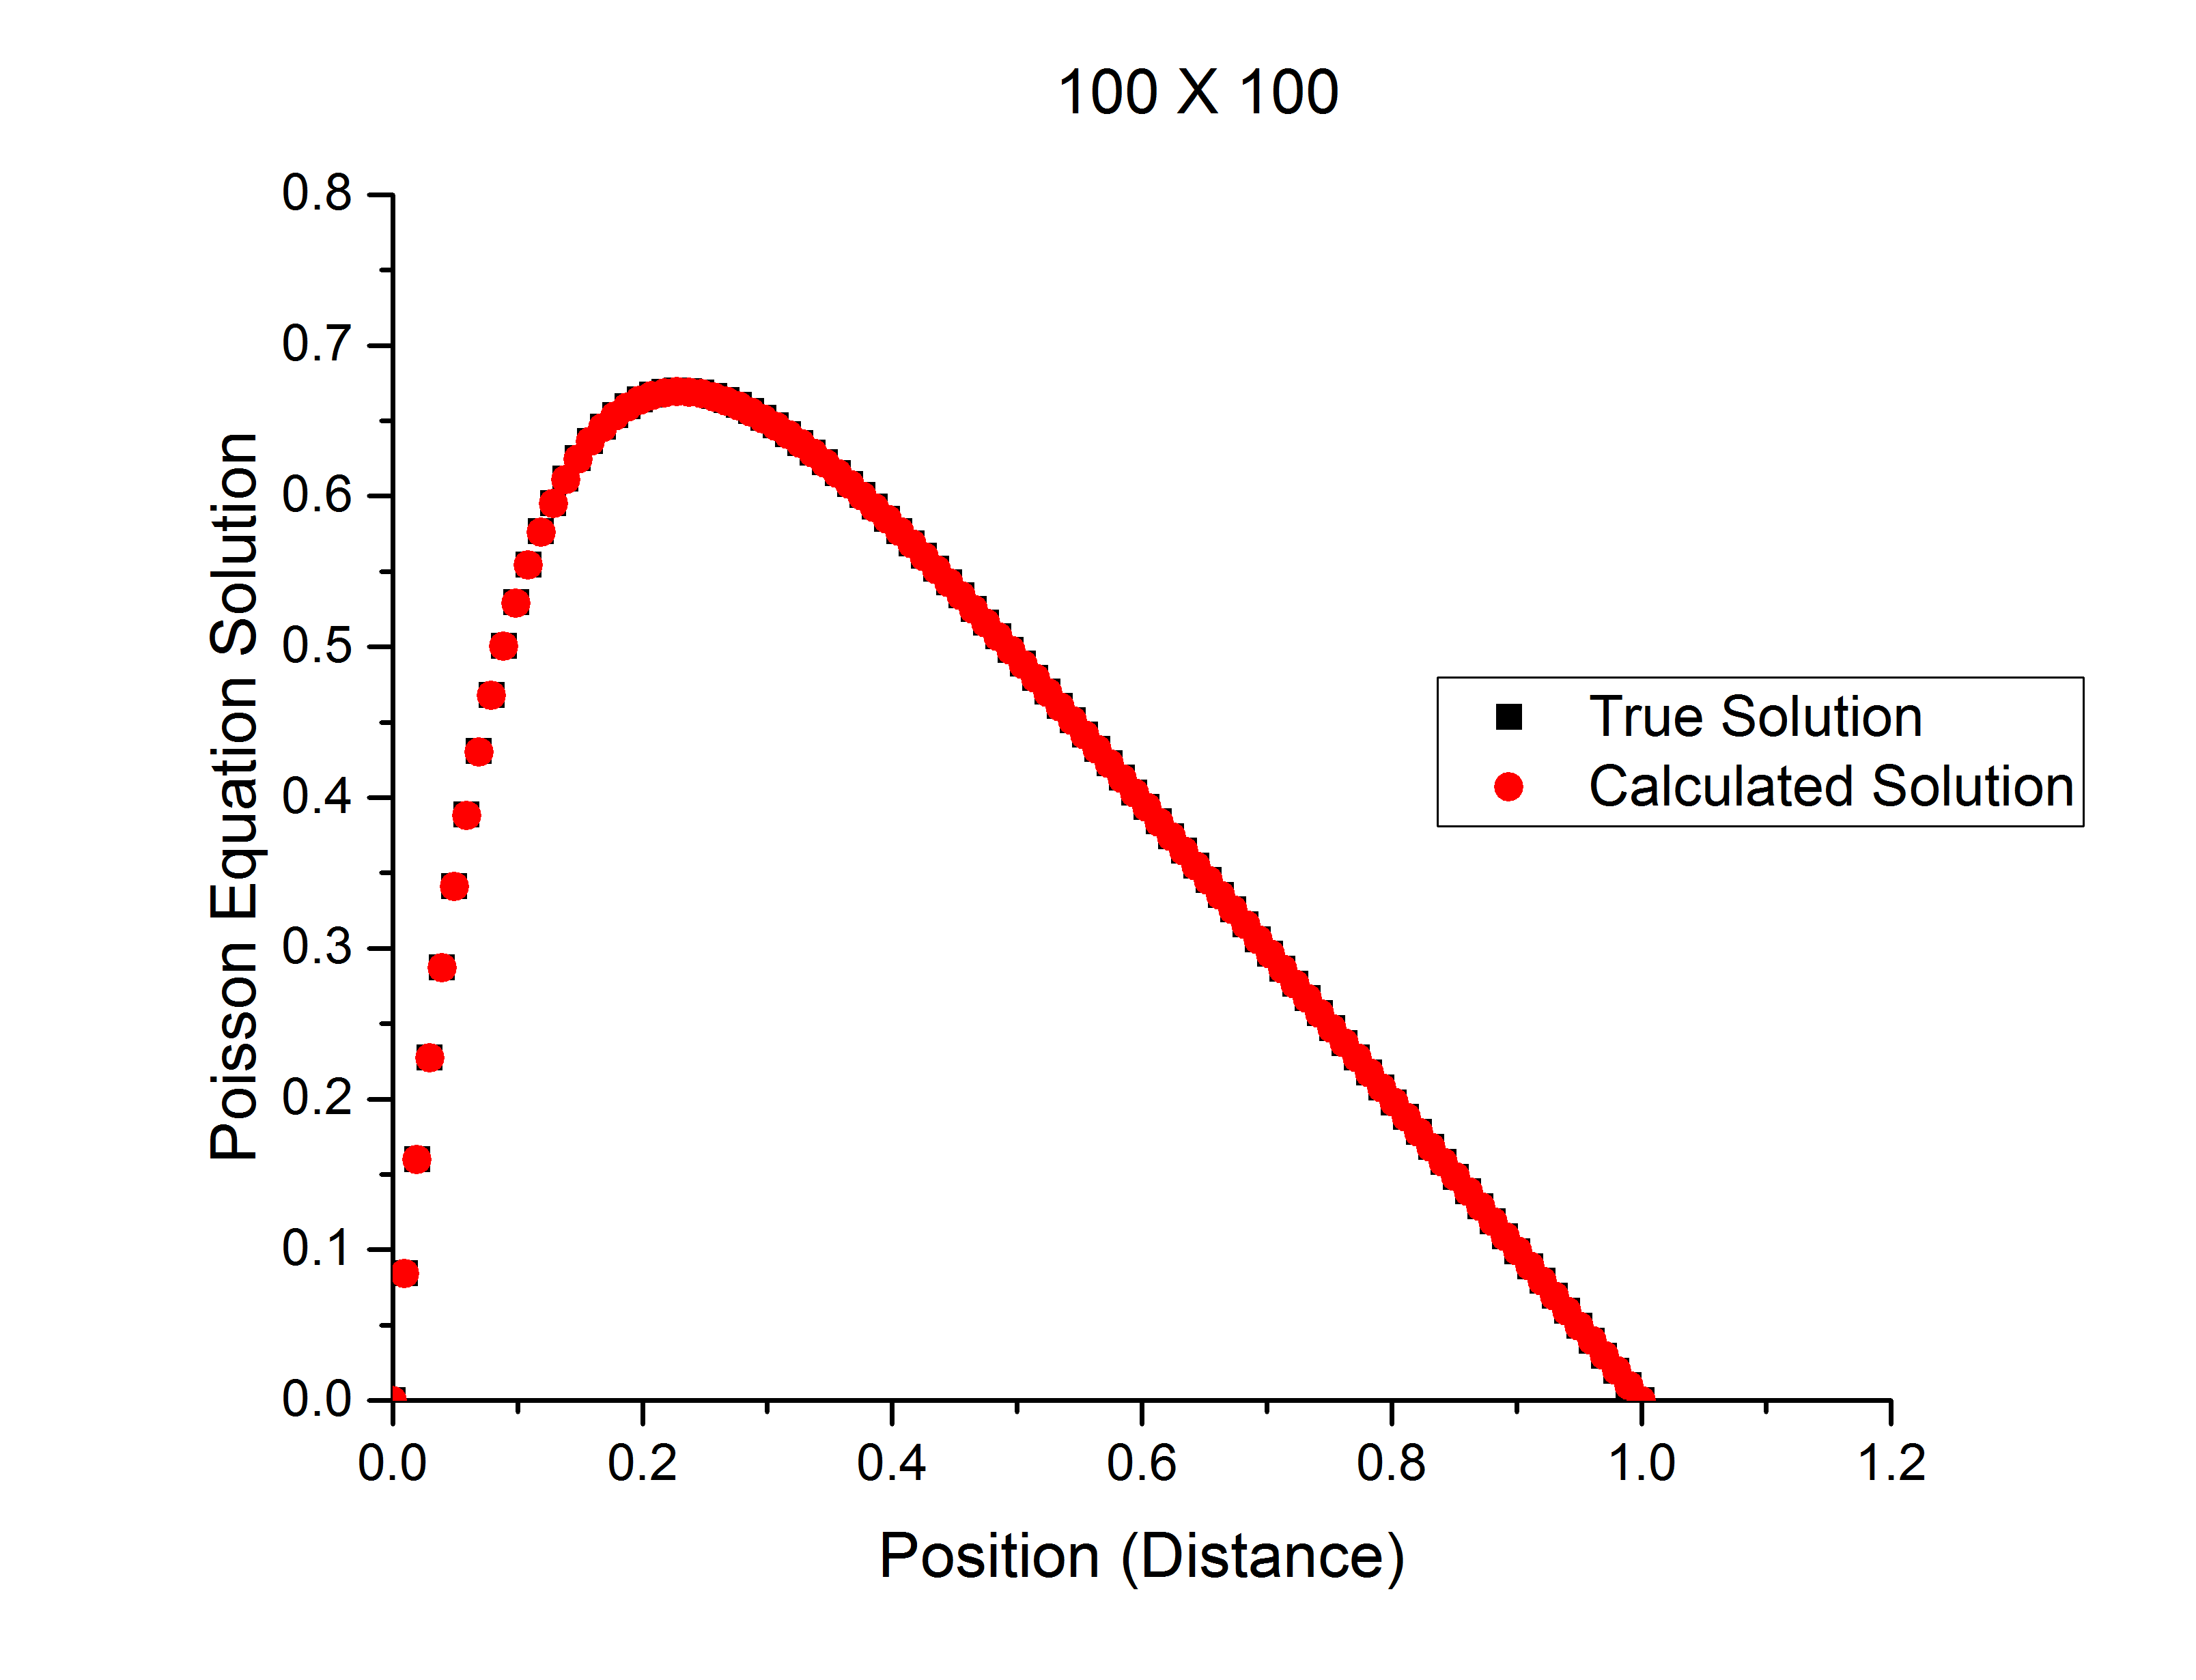
\includegraphics[scale=0.25]{100GridPoisson.png}
	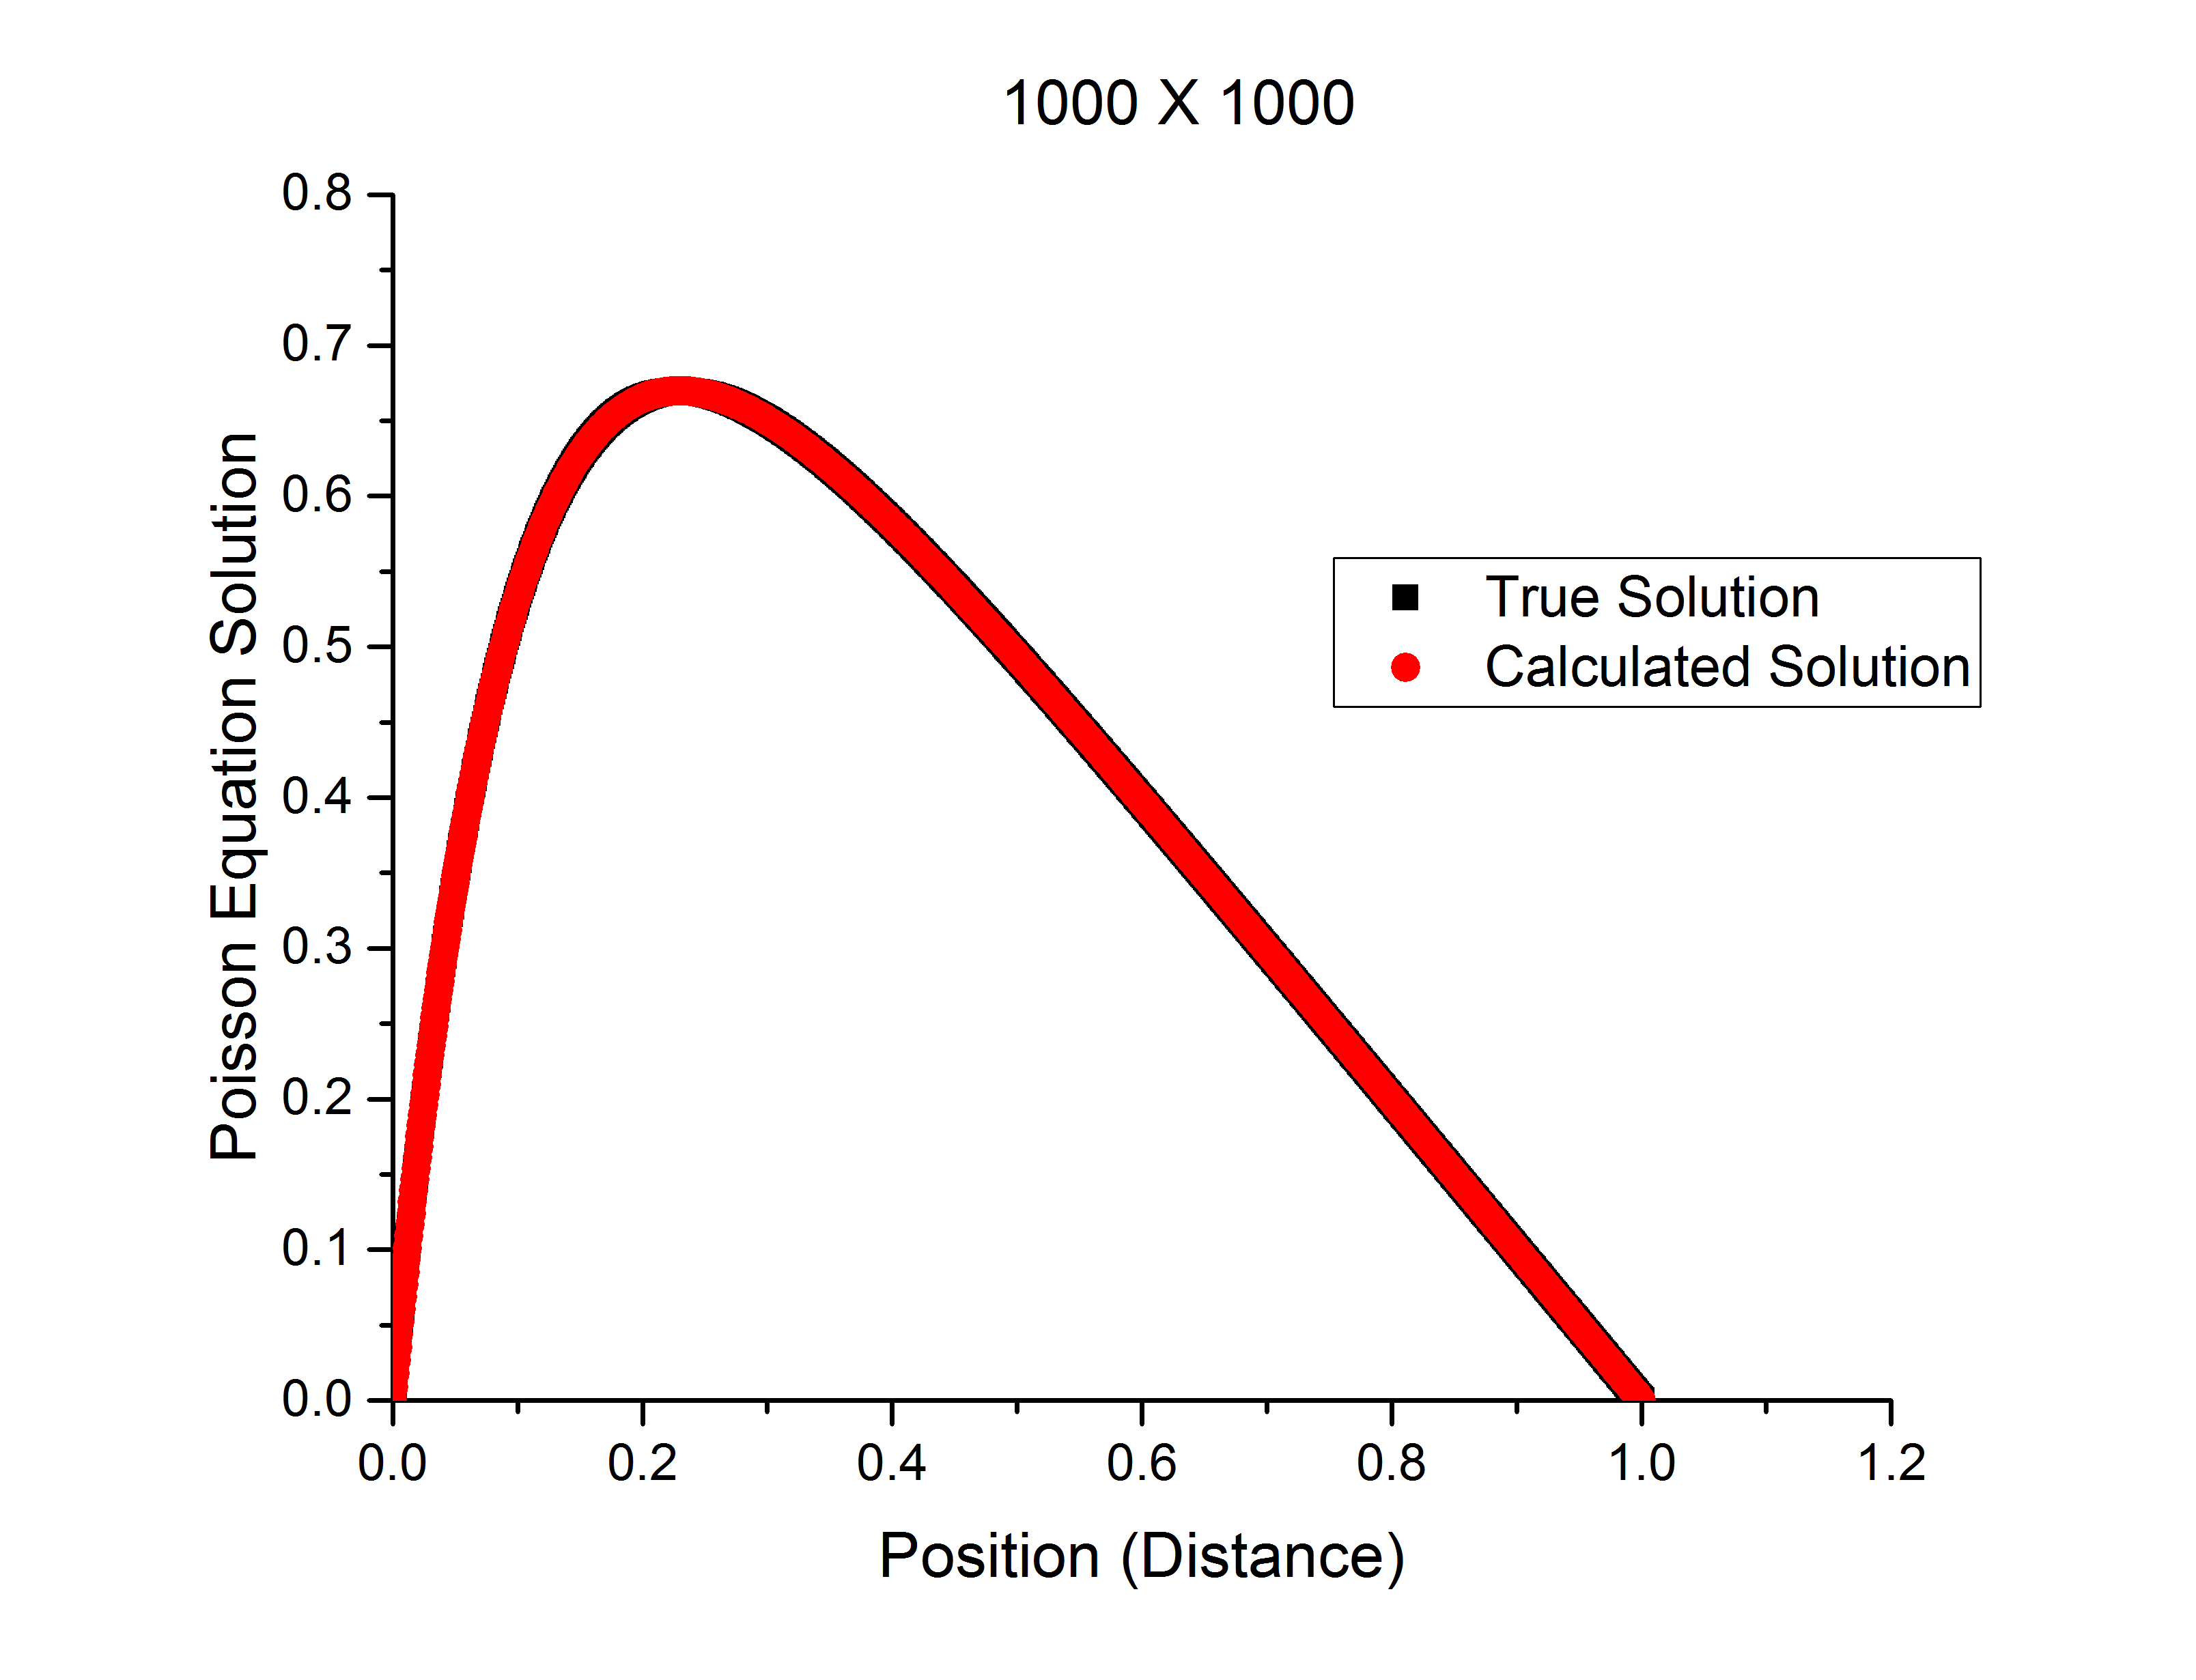
\includegraphics[scale=0.25]{1000GridPoisson.png}
	
	Figure 1: Solutions to Poisson's equation for different step sizes.
	
	
	\includegraphics[scale=0.3]{relativeerror.png}
	
	Figure 2: Relative error of Poisson's equation for different step sizes.
	
	Once solutions were found the next step was to look at the relative error for different step sizes. Figure 2 shows on a log base 10 scale the log of the relative error:
	\[\epsilon_i=\log_{10}(\frac{u_i-x_i}{x_i})\]
	Looking at figure 2 we see that the error drops as the step size decreases linearly on the log scale, this indicates it would normally go as $n^2$. This value of the minimum relative error corresponds to the step size of $\frac{1}{100000}$, after which the relative error starts to rise. More points would have been done but my computer wouldn't make arrays of 100,000,000.
	
	The final thing which was investigated was comparing the computation speed of the simple tridiagonal matrix solver presented here to the classical LU decomposition. The results were rather eye opening, as a matter of fact the LU decomposition was completely blown away. The results are presented in table 1. For the LU decomposition a matrix which was 4000 by 4000 took almost 4 minutes to run, while the tridiagonal solver took less than a second. I tried to run the LU decomposition for a matrix of 10000 but I became impatient. Even though the tridiagonal solver was much faster it will only work for very specific cases, mainly matrices which are tridiagonal. Where even though it is much slower the LU decomposition will work on non sparse matrices. The main lesson to be taken away from this is to know what your
	\begin{table}
		\caption{Computation Time for Different Differential Equation Solving Algorithms}
		\begin{tabular}{c c c}
			\hline\hline
			Matrix Size & LU Decomposition & Tridiagonal Solver \\ 
			\hline
			10 & 0 & 0 \\
			100 & 0 & 0 \\
			1000 & 2 & 0 \\
			1500 & 7 & 0 \\
			2000 & 20 & 0 \\
			2500 & 44 & 0 \\
			3000 & 83 & 0 \\
			3500 & 140 & 0 \\
			4000 & 224 & 0 \\
			10000000 & Infinity & 1 \\
			\hline
			\end{tabular}
	\end{table}
	

\section{Conclusion}
	Of the methods explored for solving Poisson's Equation using a tridiagonal solving algorithm is really the easiest way to go. This method is fast and efficient, and as shown above also very accurate even for only 100 steps. The algorithm that was used can easily be modified to accommodate other problems with sparse matrices, making it an ideal starting place for many such numerical problems. Now, the algorithm used would have problems if any of the elements in the diagonals were zero, this would cause issues with 1 being divided by 0. Luckily, this problem, if ever encountered can be handled by implementing some sort of pivoting algorithm in the code to deal with it. So, what can be taken away from this project are the following. First off methods like Gaussian Elimination and LU decomposition may work however if can be done it is simply better to try and find an alternative to these more brute force methods. Using them will take a large amount of computing time and they will not analyze extremely large systems. Secondly, using small step sizes is not the best way to get a precise answer. It will actually introduce more error into the solution and it will take the code longer to run. Finally, sparse matrices are very common in computing and it is very important to have a strong grasp on how to solve them.
	
	I would just like to say that this was a very enjoyable project and I had a lot of fun doing it.
	

\end{document}	